\documentclass{beamer}

\newcommand{\lesson}{Hashed Collections}


\newcommand{\course}{Introduction to Object-Oriented Programming}
\subject{\course}
\title[\lesson]{\course}
\subtitle{\lesson}

\author[CS 1331]
{Christopher Simpkins \\\texttt{chris.simpkins@gatech.edu}}
\institute[Georgia Tech]

\date[]{}

\newcommand{\link}[2]{\href{#1}{\textcolor{blue}{\underline{#2}}}}
\newcommand{\code}{http://www.cc.gatech.edu/~simpkins/teaching/gatech/cs1331/code}

\usepackage{colortbl}

% If you have a file called "university-logo-filename.xxx", where xxx
% is a graphic format that can be processed by latex or pdflatex,
% resp., then you can add a logo as follows:

% \pgfdeclareimage[width=0.6in]{coc-logo}{cc_2012_logo}
% \logo{\pgfuseimage{coc-logo}}

\mode<presentation>
{
  \usetheme{Berlin}
  \useoutertheme{infolines}

  % or ...

 \setbeamercovered{transparent}
  % or whatever (possibly just delete it)
}

\usepackage{tikz}
% Optional PGF libraries
\usepackage{pgflibraryarrows}
\usepackage{pgflibrarysnakes}
\usepackage{pgfplots}
\usepackage{fancybox}
\usepackage{listings}
\usepackage[abbr]{harvard}
\usepackage{hyperref}
\hypersetup{colorlinks=true,urlcolor=blue}
\usepackage[english]{babel}
% or whatever

\usepackage[latin1]{inputenc}
% or whatever

\usepackage{times}
\usepackage[T1]{fontenc}
% Or whatever. Note that the encoding and the font should match. If T1
% does not look nice, try deleting the line with the fontenc.


\usepackage{listings}

% "define" Scala
\lstdefinelanguage{scala}{
  morekeywords={abstract,case,catch,class,def,%
    do,else,extends,false,final,finally,%
    for,if,implicit,import,match,mixin,%
    new,null,object,override,package,%
    private,protected,requires,return,sealed,%
    super,this,throw,trait,true,try,%
    type,val,var,while,with,yield},
  otherkeywords={=>,<-,<\%,<:,>:,\#,@},
  sensitive=true,
  morecomment=[l]{//},
  morecomment=[n]{/*}{*/},
  morestring=[b]",
  morestring=[b]',
  morestring=[b]""",
}

\usepackage{color}
\definecolor{dkgreen}{rgb}{0,0.6,0}
\definecolor{gray}{rgb}{0.5,0.5,0.5}
\definecolor{mauve}{rgb}{0.58,0,0.82}

% Default settings for code listings
\lstset{frame=tb,
  language=scala,
  aboveskip=2mm,
  belowskip=2mm,
  showstringspaces=false,
  columns=flexible,
  basicstyle={\scriptsize\ttfamily},
  numbers=none,
  numberstyle=\tiny\color{gray},
  keywordstyle=\color{blue},
  commentstyle=\color{dkgreen},
  stringstyle=\color{mauve},
  frame=single,
  breaklines=true,
  breakatwhitespace=true,
  keepspaces=true
  %tabsize=3
}


% If you wish to uncover everything in a step-wise fashion, uncomment
% the following command:

% \beamerdefaultoverlayspecification{<+->}


\begin{document}

\begin{frame}
  \titlepage
\end{frame}


%------------------------------------------------------------------------
\begin{frame}[fragile]{The Collections Framework}

\begin{center}
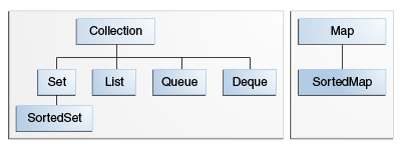
\includegraphics[width=4in]{colls-coreInterfaces.png}
\end{center}

\begin{itemize}
\item A {\it collection} is an object that represents a group of objects.
\item The collections framework allows different kinds of collections to be dealt with in an implementation-independent manner.
\end{itemize}


\end{frame}
%------------------------------------------------------------------------

%------------------------------------------------------------------------
\begin{frame}[fragile]{Well-Behaved Elements}

Collections library provides many useful implementations and algorithms.  To make maximum use of these collections, your classes should
\begin{itemize}
\item Implement {\tt Comparable<T>} so that collections whose elements are instances of your classes can be passed to algorithms that rely on the {\tt Comparable<T>} interface,
\item override {\tt equals} so that collections whose elements are instances of your classes can be queried for element membership, and
\item override {\tt hashCode} so that hash-based collections will work properly with instances of your classes.
\end{itemize}

Today we'll learn in more detail why you should override {\tt hashCode} any time you override {\tt equals}.

\end{frame}
%------------------------------------------------------------------------

%------------------------------------------------------------------------
\begin{frame}[fragile]{The {\tt equals} Method and Collections}



\begin{itemize}
\item A class whose instances will be stored in a collection must have a properly implemented {\tt equals} method.
\item The {\tt contains} method in collections uses the {\tt equals} method in the stored objects.
\item The default implementation of {\tt equals} (object identity - true only for same object in memory) only rarely gives correct results.
\item Note that {\tt hashCode()} also has a defualt implementation that uses the object's memory address.  As a rule, whenever you override {\tt equals}, you should also override {\tt hashCode}, which we'll also learn today.
\end{itemize}


\end{frame}
%------------------------------------------------------------------------

%------------------------------------------------------------------------
\begin{frame}[fragile]{{\tt equals} Method Examples}

\vspace{-.05in}
In this simple class hierarchy, {\tt FoundPerson} has a properly implemented {\tt equals} method and {\tt LostPerson} does not.
\vspace{-.05in}
\begin{lstlisting}[language=Java]
public class ArrayListEqualsDemo {
    static abstract class Person {
        public String name;
        public Person(String name) { this.name = name; }
    }
    static class LostPerson extends Person {
        public LostPerson(String name) { super(name); }
    }
    static class FoundPerson extends Person {
        public FoundPerson(String name) { super(name); }

        public boolean equals(Object other) {
            if (this == other) return true;
            if (!(other instanceof Person)) return false;
            return ((Person) other).name.equals(this.name);
        }
    }
\end{lstlisting}
\vspace{-.05in}
Examine the code in \link{\code/collections/ArrayListEqualsDemo.java}{ArrayListEqualsDemo.java} to see the consequences.

\end{frame}
%------------------------------------------------------------------------

%------------------------------------------------------------------------
\begin{frame}[fragile]{{\tt equals} and {\tt hashCode}}

{\tt java.lang.Object} has another method used by collections:
\begin{lstlisting}[language=Java]
public int hashCode()
\end{lstlisting}
\begin{itemize}
\item The {\tt hashCode} method maps an object to an {\tt int} which can be used to find the object in a kind of data structure known as a hash table.
\item Java's hash-based data structures, {\tt HashSet} and {\tt HashMap} use hash tables to store elements and keys.
\item The point of a hash code is that it can be computed in constant time, so hashtables allow very fast lookups.
\item Every object's {\tt hashCode} method should return a consistent hash code that  is not necessarily unique among all objects.
\end{itemize}

More specifically ...

\end{frame}
%------------------------------------------------------------------------

%------------------------------------------------------------------------
\begin{frame}[fragile]{{\tt hashCode}'s Contract}
\vspace{-.12in}
\begin{itemize}
\item Whenever it is invoked on the same object more than once during an execution of a Java application, the hashCode method must consistently return the same integer, provided no information used in equals comparisons on the object is modified. This integer need not remain consistent from one execution of an application to another execution of the same application.
\item If two objects are equal according to the {\tt equals(Object)} method, then calling the {\tt hashCode} method on each of the two objects must produce the same integer result.
\item It is not required that if two objects are unequal according to the {\tt equals(java.lang.Object)} method, then calling the hashCode method on each of the two objects must produce distinct integer results. However, the programmer should be aware that producing distinct integer results for unequal objects may improve the performance of hash tables.
\end{itemize}

\end{frame}
%------------------------------------------------------------------------

%------------------------------------------------------------------------
\begin{frame}[fragile]{A Correct but Terrible {\tt hashCode()}}

\begin{lstlisting}[language=Java]
public int hashCode() {
    return 1;
}
\end{lstlisting}
This {\tt hashCode} is correct because
\begin{itemize}
\item it returns the same value on subsequent invocations,
\item {\tt a.hashCode() == b.hashCode()} when {\tt a.equals(b)}, and
\item It's legal for {\tt a.hashCode() == b.hashCode()} when {\tt !a.equals(b)}.
\end{itemize}
However, the programmer should be aware that producing distinct integer results for unequal objects may improve the performance of hash tables.

\end{frame}
%------------------------------------------------------------------------

%------------------------------------------------------------------------
\begin{frame}[fragile]{A 5-Minute Introduction to Hash Tables}

\begin{itemize}
\item A hash table stores its elements in "buckets" that are addressed with {\tt int}s.
\item An object's {\tt hashCode} determines which bucket the object will be stored in.
\item Buckets are accessed very quickly, roughly as quickly as array indexing.
\item If each bucket only has one element -- because each element has a unique hash code -- then every element can be retrieved equally fast.
\item When multiple elements have the same {\tt hashCode} (a "hash collision") they go into the same bucket, which stores the elements in a linked list (which has slower access)
\end{itemize}

\end{frame}
%------------------------------------------------------------------------

%------------------------------------------------------------------------
\begin{frame}[fragile]{An Example Hash Function}

Here's a hash function based on the first letter of the name:
\begin{lstlisting}[language=Java]
public class Person {
    private String name;
    public int hashCode() { return name.charAt(0) - 'A'; }
}
\end{lstlisting}

Then Aaron, Brent, Evan and Ethan would be stored like this:
\begin{center}
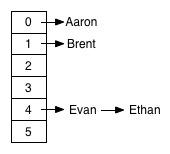
\includegraphics[height=1.5in]{hashtable.png}
\end{center}

\end{frame}
%------------------------------------------------------------------------

%------------------------------------------------------------------------
\begin{frame}[fragile]{A Legal but Bad {\tt hashCode}}

Recall our correct but terrible {\tt hashCode}:
\begin{lstlisting}[language=Java]
public int hashCode() { return 1; }
\end{lstlisting}

Using this {\tt hashCode} the hash table degenerates to a linked list:

\begin{center}
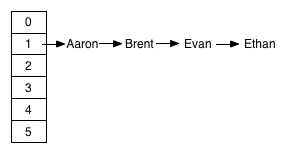
\includegraphics[height=1.5in]{hashtable-bad.png}
\end{center}

\end{frame}
%------------------------------------------------------------------------

%------------------------------------------------------------------------
\begin{frame}[fragile]{How Items are Found in a Hash-Based Collection}
\vspace{-.1in}
The item's {\tt hashCode} is used to access the right bucket, then its {\tt equals} method is used to match elements in the bucket.
\vspace{-.1in}
\begin{center}
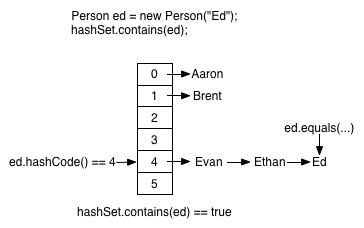
\includegraphics[height=2.5in]{hashtable-find.png}
\end{center}
\vspace{-.1in}
If you override {\tt equals}, you must override {\tt hashCode}!
\end{frame}
%------------------------------------------------------------------------


%------------------------------------------------------------------------
\begin{frame}[fragile]{A Recipe for Implementing {\tt hashCode}\footnote{Joshua Bloch, {\it Effective Java}}}
\vspace{-.05in}
You'll learn hashing in depth in your data structures and algorithms course.  For now, here's a recipe to follow:

\begin{enumerate}
\item Initialize {\tt result} with a constant non-zero value, e.g., 17
\item For each significant field {\tt f} (i.e., compared in {\tt equals} method), compute an {\tt int} hash code {\tt c} and add it to {\tt 31 * result}.
\begin{itemize}
\item For {\tt boolean} fields, \verb@c = (f ? 1 : 0)@
\item For {\tt byte, char, short, int} fields, {\tt c = (int) f}
\item For {\tt long} fields, \verb@c = (int) (f ^ (f >>> 32 ))@
\item For {\tt float} fields, {\tt c = Float.floatToIntBits(f)}
\item For {\tt double} fields, \verb@c = (int) (Double.doubleToLongBits(f) ^@ \\ \verb@    (Double.doubleToLongBits(f) >>> 32))@ \\ (notice this converts to {\tt long} then uses recipe for {\tt long} fields)
\item For reference fields, if {\tt equals} calls {\tt equals} on the field, {\tt c = f.hashCode()}
\item For array fields, {\tt c = Arrays.hashCode(f)}
\end{itemize}
\item {\tt return result}
\end{enumerate}

\end{frame}
%------------------------------------------------------------------------

%------------------------------------------------------------------------
\begin{frame}[fragile]{An Example {\tt hashCode} Using Recipe\footnote{Joshua Bloch, {\it Effective Java}}}

\begin{lstlisting}[language=Java]
class Trooper implements Comparable<Trooper> {

    private String name;
    private boolean mustached;
...
    public boolean equals(Object other) {
        if (null == other) return false;
        if (this == other) return true;
        if (!(other instanceof Trooper)) return false;
        Trooper that = (Trooper) other;
        return this.name.equals(that.name)
                && this.mustached == that.mustached;
    }
    public int hashCode() {
        int result = 17;
        result = 31 * result + name.hashCode();
        result = 31 * result + (mustached ? 1 : 0);
        return result;
    }
}
\end{lstlisting}

\end{frame}
%------------------------------------------------------------------------

%------------------------------------------------------------------------
\begin{frame}[fragile]{Consequences of Failing to Override {\tt hashCode}}

\begin{lstlisting}[language=Java]
  Set<Trooper> trooperSet = HashSet<>();
  // ...
  trooperSet.add(new Trooper("Mac", true));

  // Mac is in the set, but we don't find him because we didn't
  // override hashCode().
  System.out.println("\nOops!  Didn't override hashCode():");
  System.out.println("trooperSet.contains(new Trooper(\"Mac\", true))="
                     + trooperSet.contains(new Trooper("Mac", true)));

\end{lstlisting}
prints:
\begin{lstlisting}[language=Java]
Oops!  Didn't override hashCode():
trooperSet.contains(new Trooper("Mac", true))=false
\end{lstlisting}

Open up \link{\code/collections/SuperTroopers.java}{SuperTroopers.java} and let's fix this!

\end{frame}
%------------------------------------------------------------------------

%------------------------------------------------------------------------
\begin{frame}[fragile]{Closing Thoughts on Collections}


\begin{itemize}
\item The collections framework uses Java's OOP programming features to acheive generality and consistency.
\item Collection classes are very useful - study the Java API docs to become familiar with them.
\item In a few weeks we'll implement several basic data structures.
\begin{itemize}
\item Computer scientists need a deep understanding of data structures.
\item Application programmers should almost always use predefined data structures from the standard library.
\end{itemize}
\end{itemize}


\end{frame}
%------------------------------------------------------------------------


% %------------------------------------------------------------------------
% \begin{frame}[fragile]{}


% \begin{lstlisting}[language=Java]

% \end{lstlisting}

% \begin{itemize}
% \item
% \end{itemize}


% \end{frame}
% %------------------------------------------------------------------------


\end{document}
